\documentclass[conference]{IEEEtran}
\usepackage{cite}
\usepackage{amsmath,amssymb,amsfonts}
\usepackage{graphicx}
\usepackage{textcomp}
\usepackage{xcolor}
\usepackage{booktabs}
\usepackage{pgfplots}
\pgfplotsset{compat=1.18}
\usepgfplotslibrary{fillbetween}
\def\BibTeX{{\rm B\kern-.05em{\sc i\kern-.025em b}\kern-.08em
    T\kern-.1667em\lower.7ex\hbox{E}\kern-.125emX}}
\begin{document}

\title{Adaptive Study Planning for Self-Directed Learners: Context-Aware Pace Calibration with Change-Point Detection}

\author{
\IEEEauthorblockN{1\textsuperscript{st} ***REMOVED***}
\IEEEauthorblockA{
\textit{Dept. of Data Science and Artificial Intelligence} \\
\textit{PES University} \\
Bengaluru, India \\
***REMOVED***}
\and
\IEEEauthorblockN{2\textsuperscript{nd} Ramesh Prakash Guledgudd}
\IEEEauthorblockA{
\textit{PES University} \\
Bengaluru, India \\
rameshpg1988@gmail.com}
}

\maketitle

\begin{abstract}
Self-directed learners often begin with a fixed plan of the form ``study this many hours per day and finish by this date.'' Such a plan does not adapt when the learner's actual pace changes. This paper reports an implemented local-first study-planning prototype and the offline evaluation that shaped its adaptive components. The prototype records session events locally, sends accumulated history to a Python service for hierarchical-Bayesian pace calibration with a context-aware shrinkage override, raises a human-confirmed prompt when a single-arm CUSUM detector observes a pace shift, and projects finish dates in the client with a Gaussian-process and analytic cold-start composite. The evaluation uses synthetic learner logs with planted ground truth, calibrated against OULAD engagement moments, across 200 seeds, 5{,}400 learners, and 346{,}394 sessions in the main frozen and decoupled regimes. The context-aware calibrator lowers prospective pace-prediction error against the hierarchical-Bayesian incumbent in every decoupled-regime history band, with deltas from $-0.0145$ to $-0.0307$ and Holm correction surviving in 12/12 cells. Detection favors fast CUSUM prompting but exposes a false-alarm trade-off. Projection results show that the uncorrected Gaussian-process interval under-covers badly, while a split-conformal correction restores near-nominal coverage in research; that correction is not yet promoted into the prototype. The main limitation is that the algorithmic claims are synthetic and do not establish learning-outcome gains for real users.
\end{abstract}

\begin{IEEEkeywords}
adaptive learning, Bayesian calibration, change-point detection, Gaussian processes, study planning, self-regulated learning
\end{IEEEkeywords}

\section{Introduction}
A self-directed learner works through online courses, certification material, or examination preparation without an instructor setting the pace. Such a learner typically starts from a fixed plan of the form ``a fixed number of hours a day, finish by this date.'' The plan is a one-time estimate: it assumes the learner will study at the intended rate and that each item of material will take as long as guessed.

Within days the plan no longer matches reality. The learner falls behind on some days and gets ahead on others, the estimate for how long an item takes proves wrong, and the fixed plan never adjusts. The learner is left without a current estimate of how far off track they are or when they will actually finish, while the plan keeps displaying a stale completion date as though it were still valid.

Existing tools address only one side of this problem. Time-tracking applications record how long a learner studied but do not plan. Static plan generators, including deep-learning-plus-optimization approaches such as that of Islam et al.~\cite{islam2024}, compute a schedule once from a predicted pace and never revise it against the pace the learner actually demonstrates. Neither line of work learns the learner's realized pace as evidence accumulates, and neither revises the completion estimate in response.

The difficulty is that the evidence available to solve this problem is sparse and non-stationary. A single learner produces only a handful of sessions before a plan first needs to adapt, which rules out methods that require large per-learner samples. A learner's pace also shifts when their circumstances change, so a useful system must distinguish a persistent shift from ordinary day-to-day variation before acting on it. These two constraints, sparse evidence and non-stationary behavior, shape every design choice in the rest of this paper.

This paper makes the following contributions.
\begin{itemize}
\item A context-aware pace calibrator that augments hierarchical Bayes with 10 observable session features and population-prior shrinkage, evaluated against moving-average, EWMA, pooled-Bayes, and hierarchical-Bayes baselines.
\item A human-confirmed adaptation flow in an implemented local-first prototype: server-side pace calibration and single-arm CUSUM prompting, client-side progress projection, and capacity bookings that replace item-level day packing.
\item An offline comparison protocol over 200 seeds, held-out learner archetypes, bootstrap confidence intervals, and Holm/Benjamini--Hochberg correction, applied to calibration, detection, projection, and the retired packed-slot scheduler.
\item An evidence boundary between what is implemented and what remains research: the cold-start GP composite and enriched calibrator are promoted, while split-conformal interval correction and tuned dual-arm CUSUM remain future app work.
\end{itemize}

The remainder of this paper is organized as follows. Section~II reviews related work on pace modeling, change detection, progress projection, and adaptive scheduling. Section~III describes the system architecture. Section~IV develops the methodology, including the candidate models considered for each component and the offline comparison procedure. Section~V reports and discusses the results. Section~VI concludes and outlines future work.

\section{Related Work}
Learner pace modeling underlies any planner that adapts to an individual. Chen et al.~\cite{chen2024} present a hierarchical Bayesian model of adaptive teaching, validated across two behavioral experiments with 312 adults, and show that hierarchical priors capture learner-to-learner variability without overfitting to sparse per-learner data, which is the statistical basis for estimating a pace from a handful of sessions. Zambrano et al.~\cite{zambrano2024} analyze algorithmic bias in Bayesian Knowledge Tracing at scale and find performance essentially equal across demographic groups, supporting the reliable use of Bayesian-family models across diverse learners. Mai et al.~\cite{mai2025} couple deep temporal modeling with a probabilistic layer in a Transformer--Bayesian hybrid that recovers interpretable, calibrated estimates. These works establish Bayesian calibration as sound for learner modeling, but they target correctness or mastery prediction rather than the planned-versus-actual pace estimation this paper requires.

Detecting a persistent shift in a learner's behavior is what makes timely replanning possible. Saqr et al.~\cite{saqr2026} apply critical-slowing-down indicators to 1.67~million practice attempts from 9{,}401 students and find that 88.2\% of disengaging learners show a detectable warning signal beforehand, evidence that per-learner behavioral shifts are recoverable from trace data. Qiao et al.~\cite{qiao2026} survey statistical-process-control methods and document the CUSUM and EWMA control-chart family that the detector in this paper builds on, though their reviewed applications are drawn from manufacturing rather than education. Neither line of work prescribes a corrective action once a shift is detected, which is the step this paper adds by feeding a detected shift into a recalibration prompt.

Projecting a completion date with a calibrated uncertainty band, rather than a bare point estimate, makes the estimate usable for planning. P\'erez-Suay et al.~\cite{perezsuay2024} apply Gaussian-process regression with an automatic-relevance-determination kernel to learning-management-system logs and report a correlation of $R=0.89$ for predicting student marks. Lin et al.~\cite{lin2024} scale Gaussian processes to learning-curve prediction with a latent Kronecker structure, matching Transformer-level accuracy while retaining calibrated uncertainty. Both works apply Gaussian-process regression cross-sectionally to a final outcome, rather than to the running, longitudinal burn-up projection this paper needs.

Islam et al.~\cite{islam2024} couple an artificial neural network for grade prediction with dynamic programming for schedule optimization, establishing the predict-then-optimize architecture this paper adopts and extends. Their generated schedule, like other adaptive-scheduling work, is solved once from a predicted pace and does not revise itself against the pace the learner goes on to demonstrate; closing that loop is a central contribution of this paper.

Self-regulated-learning analytics grounds the choice of feedback metrics for a planner that reports back to the learner. Alhazbi et al.~\cite{alhazbi2024} review 25 empirical studies measuring self-regulated learning from trace data and find that most validated indicators relate to time-management skill, which motivates this paper's use of schedule adherence as a behavioral signal. de~Barba et al.~\cite{debarba2025} develop and validate a learning-analytics rubric that maps validated self-regulation scales onto learning-management-system indicators in a scalable way. These works supply validated, trace-based indicators of self-regulation, but none feeds the signal back into an adaptive plan, which is the loop this paper closes.

Across these threads, calibration, detection, projection, and scheduling are each studied in isolation: no reviewed system integrates all four into a single adaptive loop that is evaluated end to end and implemented as a local-first study-planning prototype. This is the gap the present work addresses.

\section{System Architecture}
\begin{figure*}[!t]
\centering
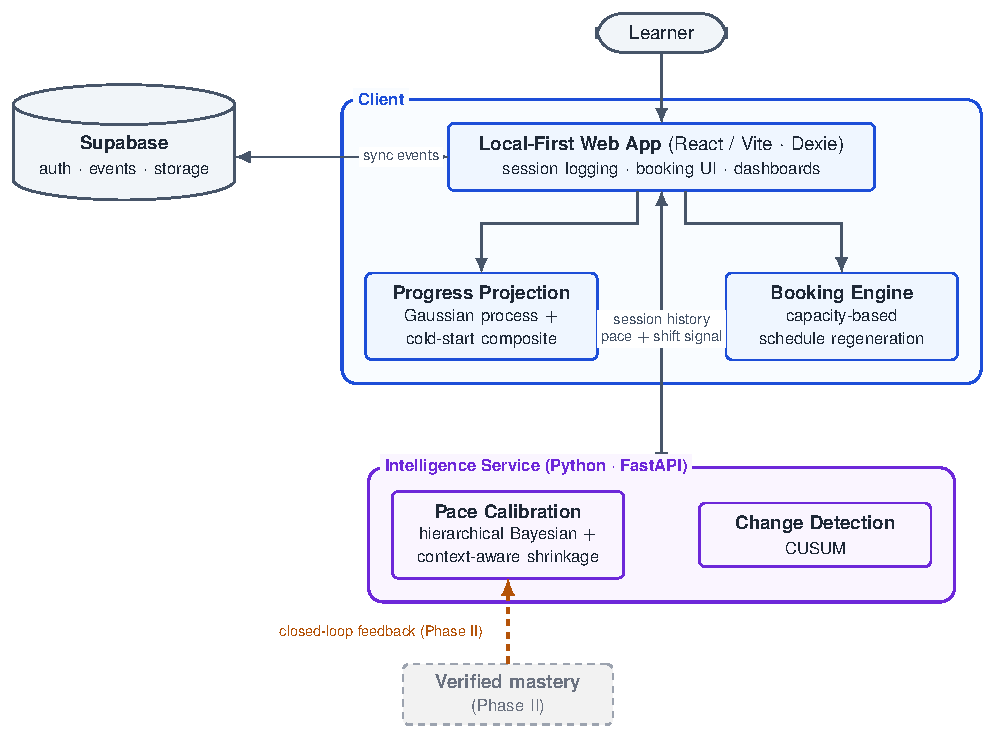
\includegraphics[width=0.8\textwidth]{fig_architecture.pdf}
\caption{Implemented prototype architecture. The client owns local event capture, booking interaction, the Gaussian-process plus analytic cold-start projection, and capacity bookings. The Python/FastAPI Intelligence Service fits the accumulated-history models used live: hierarchical Bayesian calibration with a context-aware shrinkage override and single-arm CUSUM prompting. Supabase supports authentication, persisted user data, and snapshots. Split-conformal interval correction and verified-mastery feedback are research or Phase-II work, not current prototype behavior.}
\label{fig:arch}
\end{figure*}
The implemented prototype is organized into two tiers of computation around a data hub, with the split between them decided by a simple rule: computation that fits a statistical model to accumulated history runs on the server, and computation that derives a view directly from the learner's local event log runs on the client. Fig.~\ref{fig:arch} shows the resulting architecture.

The client is a local-first single-page application built with React and Vite, storing learner actions as events in a per-user IndexedDB store through Dexie. It owns the session-logging and booking interfaces, the dashboards, the Gaussian-process progress projection with its analytic cold-start fallback, and the capacity-based booking engine. Running these client-side keeps the core loop responsive and available offline. The Intelligence Service is a Python and FastAPI application that hosts pace calibration and change detection: on each request it receives the learner's session history over an authenticated HTTP call and returns a calibrated pace multiplier together with a change-detection signal. Every request carries a token issued at sign-in, which the service verifies before any model runs. Supabase sits between the client and the service as the data hub for authentication, persisted user data, and snapshots; the evaluation claims in this paper do not depend on real cloud user logs. The closed-loop feedback from a verified-mastery signal back into calibration, shown dashed in Fig.~\ref{fig:arch}, is the principal Phase-II extension and is not part of the implemented prototype.

This architecture is the outcome of a design revision, not the first design tried. The starting point followed the predict-then-optimize architecture of Islam et al.~\cite{islam2024} literally: a predictive model estimated the learner's pace and a constraint-based optimizer packed each item of study material onto a specific calendar day, producing a dated slot grid that a replan re-computed in full. In the prototype this created concrete boundary cases. A missed booking, a partially completed item crossing a day boundary, or a small pace change could force many material assignments to move even when the learner only needed a new estimate of available study capacity. The scheduling question was therefore re-examined, and the prescriptive packer was replaced with the capacity-based booking model in Fig.~\ref{fig:arch}: the plan holds blank bookings, each carrying a date and a duration, and the learner chooses the specific material at the start of a session. The pace-calibration, change-detection, and projection models were confirmed to transfer to the revised design (Section~V), so the redesign changed how a plan is represented, not what is estimated about the learner.

\section{Methodology}
Each component was chosen by comparing candidate models offline against established baselines rather than by assumption, using the procedure of Section~\ref{sec:method-compare}. Table~\ref{tab:candidates} summarizes the candidates considered per component and the approach used in the implemented prototype.

\begin{table*}[!t]
\centering
\caption{Candidate models per component and the approach used in the implemented prototype.}
\label{tab:candidates}
\begin{tabular}{p{2.6cm} p{7.6cm} p{6.4cm}}
\toprule
\textbf{Component} & \textbf{Candidates compared} & \textbf{Approach used in the implemented prototype} \\
\midrule
Pace calibration & Moving average, EWMA, pooled Bayesian, hierarchical Bayesian, context-aware shrinkage & Hierarchical Bayesian posterior (Eq.~\eqref{eq:bayes-update}) refined by the context-aware shrinkage calibrator (Eq.~\eqref{eq:enriched}) \\
Change detection & CUSUM, EWMA control chart, critical slowing down, Page--Hinkley, Bayesian online change-point, ADWIN & CUSUM change-point detection (Eq.~\eqref{eq:cusum}); the fastest detector, feeding a human-confirmed recalibration prompt \\
Progress projection & Linear extrapolation, Gaussian process, GP with cold-start composite, split-conformal interval correction & Gaussian process (Eq.~\eqref{eq:gp-kernel}) with a cold-start analytic composite; split-conformal correction is evaluated but not yet promoted \\
Schedule generation & Rule-based, dynamic-programming capacity allocator (Eq.~\eqref{eq:dp}), greedy prerequisite-aware, local-search repair & Not adopted; day-by-day packing was replaced by the capacity-based booking model of Section~III following the evaluation in Section~\ref{sec:res-sched} \\
\bottomrule
\end{tabular}
\end{table*}

\subsection{Pace Calibration}
\label{sec:method-cal}
For a session $t$, let the pace ratio be $r_t = a_t/p_t$, the ratio of active minutes $a_t$ to planned minutes $p_t$, modeled as $r_t \sim \mathcal{N}(\mu,\sigma^2)$ with prior $\mu \sim \mathcal{N}(\mu_0,\tau_0^2)$ centered at $\mu_0=1$. With $n$ observed sessions the conjugate posterior is Gaussian,
\begin{equation}
\begin{split}
p(\mu \mid r_{1:n}) &= \mathcal{N}(\mu_n,\tau_n^2), \\
\tau_n^2 &= \Big(\tfrac{1}{\tau_0^2}+\tfrac{n}{\sigma^2}\Big)^{-1}, \\
\mu_n &= \tau_n^2\Big(\tfrac{\mu_0}{\tau_0^2}+\tfrac{1}{\sigma^2}\sum_{t=1}^{n} r_t\Big).
\end{split}
\label{eq:bayes-update}
\end{equation}
This hierarchical Bayesian posterior is the incumbent: it stays close to the prior while $n$ is small, which is what makes a usable estimate available from a handful of sessions, and tightens around the learner's realized rate as $n$ grows.

The implemented service refines this estimate with a context-aware shrinkage calibrator. Let $\phi_t \in \mathbb{R}^d$ be a vector of observable session context, covering intercept, anchor role, practice role, morning, evening, weekend, same-day extra session, planned progress, deadline urgency, and recency, and let $y_t = \log(a_t/p_t)$ be the log pace ratio. The calibrator fits weights $w$ by ridge-regularized least squares shrunk toward a population prior $w_0$ rather than toward zero,
\begin{equation}
\hat{w} = \arg\min_{w}\ \sum_t \big(y_t - w^{\top}\phi_t\big)^2 \; + \; \lambda\,\lVert w \rVert^2 \; + \; \gamma\,\lVert w - w_0 \rVert^2,
\label{eq:enriched}
\end{equation}
with ridge strength $\lambda=2.0$ and population-prior shrinkage strength $\gamma=6.0$ in the promoted implementation. The pace multiplier for a context $\phi$ is $\exp(\hat{w}^{\top}\phi)$. Shrinking toward a population prior, rather than toward zero, lets the model behave sensibly when a learner has logged few sessions and converge to learner-specific behavior as sessions accumulate. The service refits the model on each calibration request rather than persisting model state. The promoted calibrator is an ensemble of two such models, seeded with different population priors and combined by leave-one-out-weighted averaging, with fixed fallback weights when fewer than two sessions are available.

\subsection{Change Detection}
\label{sec:method-det}
A one-sided cumulative-sum chart tracks the running deviation of the pace signal $x_t$ from its in-control mean $\mu_0$,
\begin{equation}
S_0 = 0, \qquad S_t = \max\!\big(0,\; S_{t-1} + (x_t-\mu_0) - k\big),
\label{eq:cusum}
\end{equation}
and the chart raises an alarm once $S_t > h$, where the slack $k$ absorbs ordinary day-to-day variation and $h$ is the decision threshold~\cite{qiao2026}. The statistic stays near zero while the pace is stable and accumulates once a persistent shift occurs. A detected shift raises a recalibration prompt; the learner confirms or dismisses the prompt before any replan action (Section~\ref{sec:res-det}).

\subsection{Progress Projection}
\label{sec:method-proj}
A Gaussian process places a prior over progress curves and conditions it on the observed cumulative-progress points, under a squared-exponential kernel with signal variance $\sigma_f^2$ and length scale $\ell$,
\begin{equation}
k(x,x') = \sigma_f^2 \exp\!\Big(-\tfrac{(x-x')^2}{2\ell^2}\Big).
\label{eq:gp-kernel}
\end{equation}
The resulting predictive variance supplies an interval around the projected completion date, rather than a single point. The implemented client projection uses this Gaussian process with a cold-start composite: while fewer than five sessions have accumulated, or when the fitted GP would cross implausibly, it falls back to an analytic required-rate estimate. A split-conformal correction of the interval width is evaluated in Section~\ref{sec:res-proj}; it restores nominal coverage in research but is not yet part of the client implementation.

\subsection{Schedule Generation}
\label{sec:method-sched}
Writing $V(t,\rho)$ for the best achievable cost from day $t$ onward with remaining work $\rho$, a day-by-day scheduler solves a recurrence of the form
\begin{equation}
V(t,\rho) = \min_{0 \le a \le c_t}\ \big[\, \ell(a) + V(t+1,\ \rho - a)\,\big],
\label{eq:dp}
\end{equation}
where $a$ is the study time allocated on day $t$, $c_t$ is that day's capacity, and $\ell$ penalizes deadline drift~\cite{islam2024}. Section~\ref{sec:res-sched} reports that this allocator minimizes deadline drift among the scheduling candidates; Section~III records why the implemented prototype does not use it, replacing day-by-day packing with the capacity-based booking model instead.

\subsection{Offline Evaluation Dataset}
\label{sec:method-data}
The offline evaluation uses synthetic learner logs because the target quantities are not directly observable in real usage. Planted ground truth supplies each learner's pace, change schedule, and finish date, making pace recovery, detection latency, and interval coverage measurable. The synthetic generator was calibrated against Open University Learning Analytics Dataset (OULAD) engagement moments by aggregating \emph{studentVle.sum\_click} by learner, course, and day. OULAD was used as a bounded proxy for engagement intensity, not as direct validation of this prototype. The calibration pass saw 10{,}655{,}280 OULAD rows, retained 571{,}356 after filtering, and produced 1{,}440 usable learner-course series.

The main algorithm comparisons use two 5{,}400-learner regimes: a frozen anchor and a decoupled regime that models the later booking design with ad-hoc and interrupted sessions. Both contain 200 seeds, 9 learner archetypes, 3 history bands, and 346{,}394 generated sessions. The scheduling comparison uses an earlier 3{,}600-learner reality-matched regime because the packed-slot scheduling question was retired before the decoupled booking regime existed. Table~\ref{tab:eval-config} summarizes the stamped configuration.

\begin{table}[!t]
\centering
\caption{Offline evaluation configuration extracted from result manifests and synthetic JSONL files.}
\label{tab:eval-config}
\scriptsize
\begin{tabular}{p{2.45cm} p{4.55cm}}
\toprule
\textbf{Item} & \textbf{Value} \\
\midrule
Main regimes & Frozen and decoupled, each with 200 seeds, 5{,}400 learners, and 346{,}394 sessions \\
Scheduling regime & Reality-matched packed-slot regime, 200 seeds, 3{,}600 learners, and 230{,}469 sessions \\
History bands & Small, medium, and max; generated sessions per learner have min/median/max 8/53/160 \\
Archetypes & 9 for calibration, detection, and projection; 6 for scheduling \\
Held-out protocol & 5 train archetypes and 4 held-out archetypes; scoring uses the held-out split \\
Decoupled events & 51{,}813 ad-hoc sessions and 69{,}436 interrupted sessions \\
OULAD moment bounds & Gap days p50/p75/p90/p95 = 1/3/6/11; dropout probability range 0.140--0.290; shift frequency range 0.25--20 per 100 days \\
Corrections & Learner-level bootstrap delta intervals; Holm-Bonferroni primary correction; Benjamini--Hochberg reported \\
Oracle & Uses planted ground truth as an upper-bound reference; not a deployable method \\
\bottomrule
\end{tabular}
\end{table}

\subsection{Comparison Methodology}
\label{sec:method-compare}
Each candidate was evaluated offline on the datasets summarized in Table~\ref{tab:eval-config}. Candidates were evaluated on held-out learner archetypes absent from the set used to develop them, so that a win reflects generalization rather than fitting to the evaluation cases. Every reported comparison carries a bootstrap confidence interval on the difference between a candidate and the incumbent, estimated by resampling learners with replacement, and a Holm or Benjamini--Hochberg correction is applied across the family of comparisons. An oracle baseline, given the planted ground truth, is included in the results that follow as an upper-bound reference; it is never treated as a deployable method.

\section{Results and Discussion}
All results below are computed on the synthetic ground-truth datasets described in Section~\ref{sec:method-data}. Calibration and projection are reported for both the frozen synthetic regime and the decoupled regime that matches the capacity-based booking model, so that transfer across the redesign is visible. Scheduling is reported only for the earlier packed-slot regime, since the scheduling formulation was retired before the decoupled booking regime existed. Throughout, the oracle is an upper-bound reference given the planted ground truth; it is never a deployable method.

\subsection{Pace Calibration}
\label{sec:res-cal}
Two calibration metrics were separated. Recovery error measures how closely an estimate reconstructs the planted pace after the fact. Prospective context-prediction error measures the next-session pace estimate used by the planner. On recovery error, no structured Bayesian candidate consistently improves over the hierarchical-Bayesian incumbent, and the incumbent remains strongest among deployable methods at the longest histories. On prospective context prediction, the context-aware shrinkage calibrator improves over the incumbent across every history-length band and across both synthetic regimes (Table~\ref{tab:res-cal}). This is the low-data regime in which a new learner first needs the plan to adapt, so the prospective result determined the promoted calibration path.

\begin{table}[!t]
\centering
\caption{Shrinkage minus hierarchical-Bayesian prospective error; negative favors shrinkage.}
\label{tab:res-cal}
\scriptsize
\begin{tabular}{@{}l c c@{}}
\toprule
\textbf{Band} & \textbf{Frozen $\Delta$} & \textbf{Decoupled $\Delta$} \\
\midrule
Short & $-0.0148$ [$-0.0168,-0.0127$] & $-0.0145$ [$-0.0155,-0.0136$] \\
Medium & $-0.0262$ [$-0.0282,-0.0243$] & $-0.0268$ [$-0.0277,-0.0258$] \\
Long & $-0.0300$ [$-0.0316,-0.0285$] & $-0.0307$ [$-0.0316,-0.0299$] \\
\bottomrule
\end{tabular}
\end{table}

Table~\ref{tab:res-cal-ablation} expands the calibration comparison into an ablation-style view for the decoupled regime. It should be read as a candidate-family comparison, not a strict causal ablation, because some rows change more than one design choice at once. The main pattern is that context features matter: context-aware rows reduce prospective error relative to SMA, EWMA, pooled Bayes, and hierarchical Bayes in all three bands. The empirical-Bayes partial-pooling row is lowest on these decoupled prospective means, but it was not the promoted implementation because the broader frozen and reality-matched protocol, including recovery-error checks, produced significant losses for the structured covariate and EB story. The promoted \textit{enriched\_shrink}/dual-prior path is therefore the production-stable result, while this table records the useful follow-up finding that context grouping deserves further investigation.

\begin{table*}[!t]
\centering
\caption{Decoupled-regime ablation-style comparison for prospective context-prediction error. Lower is better.}
\label{tab:res-cal-ablation}
\scriptsize
\begin{tabular}{@{}l l l l c r r r@{}}
\toprule
\textbf{Candidate} & \textbf{Model role} & \textbf{Context} & \textbf{Prior/pooling} & \textbf{Ens.} & \textbf{Short} & \textbf{Medium} & \textbf{Long} \\
\midrule
SMA & Windowed mean & None & None & No & 0.07070 & 0.06258 & 0.05831 \\
EWMA & Exponential mean & None & Prior start & No & 0.07083 & 0.06320 & 0.06076 \\
Pooled Bayes & Pooled posterior & None & Bayesian prior & No & 0.07099 & 0.06772 & 0.06378 \\
Hierarchical Bayes & Incumbent & None & Hierarchical prior & No & 0.07099 & 0.06772 & 0.06378 \\
Covariate Bayes & Ridge context model & Role/time/day & Ridge & No & 0.05422 & 0.03740 & 0.02780 \\
EB partial pool & Context grouping & Role/time/day & Empirical Bayes & No & 0.03636 & 0.02258 & 0.01512 \\
Enriched shrink & Promoted base & 10 features & Population prior & No & 0.05646 & 0.04096 & 0.03307 \\
Dual prior & Promoted ensemble & 10 features & Dual priors & Yes & 0.05646 & 0.04096 & 0.03307 \\
\bottomrule
\end{tabular}
\end{table*}

\subsection{Change Detection}
\label{sec:res-det}
Table~\ref{tab:res-det} reports the decoupled-regime detector comparison. CUSUM has the lowest latency on both step and drift shifts and wins the selection score in this regime, but it also produces more false alarms than CSD, EWMA, BOCPD, or ADWIN. This is a user-experience trade-off, not a free improvement: in the prototype, a detected shift raises a prompt rather than automatically changing the plan, so a false alarm can be dismissed, but frequent prompts would still need throttling or tuning in real use. The implemented detector is a simpler single-arm CUSUM; the benchmark's tuned dual-arm CUSUM is future promotion work.

\begin{table*}[!t]
\centering
\caption{Decoupled-regime change-detection results. False alarms are rates; lower latency and lower score are better.}
\label{tab:res-det}
\scriptsize
\begin{tabular}{l r r r r r r r r}
\toprule
\textbf{Detector} & \textbf{Step lat.} & \textbf{Step FA} & \textbf{Step miss} & \textbf{Step score} & \textbf{Drift lat.} & \textbf{Drift FA} & \textbf{Drift miss} & \textbf{Drift score} \\
\midrule
ADWIN & $\infty$ & 0.000 & 200 & $\infty$ & $\infty$ & 0.000 & 600 & $\infty$ \\
BOCPD & 13.052 & 0.005 & 142 & 14213.169 & 8.746 & 0.006 & 123 & 12308.901 \\
CSD & 4.670 & 0.049 & 3 & 305.902 & 5.320 & 0.033 & 166 & 16606.138 \\
CUSUM & 1.375 & 0.180 & 0 & 5.869 & 2.294 & 0.192 & 2 & 207.095 \\
EWMA chart & 6.317 & 0.030 & 20 & 2007.062 & 7.007 & 0.031 & 66 & 6607.791 \\
Page--Hinkley & 3.055 & 0.138 & 0 & 6.503 & 2.500 & 0.125 & 42 & 4205.613 \\
\bottomrule
\end{tabular}
\end{table*}

\subsection{Progress Projection}
\label{sec:res-proj}
The raw Gaussian-process interval under-covers severely: against a nominal 95\% coverage, the plain interval covers only 18\% to 49\% of cases depending on the history-length band in the decoupled regime (Table~\ref{tab:res-proj}), and a similar shortfall appears in the frozen regime (Fig.~\ref{fig:coverage}). The cold-start composite improves the small-band case and is the projection refinement currently implemented in the client. The split-conformal correction addresses a different failure mode: it widens the interval to restore near-nominal coverage while leaving the point estimate unchanged. In the decoupled regime it restores coverage to roughly 98.8\%--98.9\%, but with much wider intervals; this correction remains a research result and future app-promotion item.

\begin{table*}[!t]
\centering
\caption{Decoupled-regime projection results. Entries are coverage / mean absolute finish-date error / interval sharpness in days. Nominal coverage is 0.95.}
\label{tab:res-proj}
\scriptsize
\begin{tabular}{l c c c}
\toprule
\textbf{Method} & \textbf{Small history} & \textbf{Medium history} & \textbf{Long history} \\
\midrule
Plain GP & 0.494 / 2.361 / 1.649 & 0.277 / 15.331 / 4.715 & 0.183 / 39.530 / 7.955 \\
GP plus analytic cold start & 0.552 / 2.139 / 2.278 & 0.291 / 17.099 / 6.222 & 0.195 / 52.105 / 10.707 \\
GP plus conformal correction & 0.989 / 2.361 / 29.408 & 0.988 / 15.331 / 119.444 & 0.988 / 39.530 / 292.293 \\
\bottomrule
\end{tabular}
\end{table*}

\begin{figure}[!t]
\centering
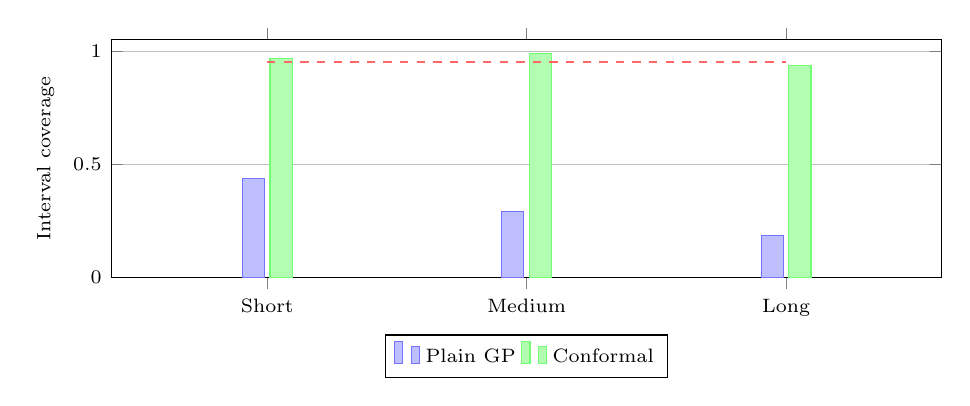
\begin{tikzpicture}
\begin{axis}[ybar, bar width=8pt, width=\linewidth, height=4.6cm, ymin=0, ymax=1.05,
  ylabel={Interval coverage}, symbolic x coords={Short, Medium, Long}, xtick=data,
  legend style={at={(0.5,-0.24)}, anchor=north, legend columns=-1, font=\scriptsize},
  ymajorgrids, enlarge x limits=0.3, label style={font=\scriptsize}, tick label style={font=\scriptsize}]
\addplot[fill=blue!25, draw=blue!55] coordinates {(Short,0.438) (Medium,0.291) (Long,0.187)};
\addlegendentry{Plain GP}
\addplot[fill=green!30, draw=green!55] coordinates {(Short,0.969) (Medium,0.990) (Long,0.937)};
\addlegendentry{Conformal}
\draw[dashed, thick, red!60] (axis cs:Short,0.95) -- (axis cs:Long,0.95);
\end{axis}
\end{tikzpicture}
\caption{Interval coverage against the nominal 0.95 (dashed) by history-length band, frozen synthetic regime. The plain Gaussian-process interval under-covers badly; the split-conformal research candidate restores near-nominal coverage but is not yet promoted into the prototype.}
\label{fig:coverage}
\end{figure}

\subsection{Schedule Generation}
\label{sec:res-sched}
Among the packed-slot scheduling candidates, the dynamic-programming capacity allocator of Eq.~\eqref{eq:dp} minimizes deadline drift in every material mix tested (Table~\ref{tab:res-sched}). Its margin over a greedy incumbent grows sharply as more material roles are interleaved: on the most demanding mix, the greedy incumbent drifts by roughly 39 days while the dynamic-programming allocator drifts by about 8, a difference of $-30.9$ days [$-31.7,-30.2$] under a 95\% bootstrap interval. This is a statistically clear result for the retired packed-slot formulation, not behavior of the current prototype. As Section~III records, the day-by-day packing formulation these schedulers share was replaced by the capacity-based booking model before the revised synthetic regime existed; the comparison is therefore reported as an evaluated result that informed a design decision.

\begin{table}[!t]
\centering
\caption{Packed-slot scheduling results from the retired scheduling formulation. Drift is mean absolute deadline drift in days.}
\label{tab:res-sched}
\scriptsize
\begin{tabular}{l r r r}
\toprule
\textbf{Material mix} & \textbf{Greedy} & \textbf{DP} & \textbf{$\Delta$} \\
\midrule
Anchor & 3.113 & 1.732 & -1.209 \\
Anchor+foundation & 3.647 & 2.353 & -1.065 \\
Anchor+practice & 5.941 & 3.912 & -2.033 \\
All roles & 38.975 & 8.297 & -30.928 \\
\bottomrule
\end{tabular}
\end{table}

\subsection{Discussion}
\label{sec:res-discuss}
The evaluation changed the system in two ways. First, it shifted the calibration criterion from retrospective recovery to prospective prediction. Recovery error is useful for diagnosis, but the planner acts on the next estimate it shows the learner. The context-aware shrinkage result is therefore most relevant in the small-history setting, where a learner has logged few sessions and the plan has the least evidence.

Second, the comparison exposed where the prototype should stay conservative. CUSUM is fast, but the false-alarm rates in Table~\ref{tab:res-det} are high enough that prompts must remain dismissible and should be rate-limited before real use. The Gaussian-process interval is useful as a point-projection mechanism, but its uncorrected uncertainty band is not calibrated; a production interval should not be presented as reliable until the conformal correction or an equivalent calibration step is promoted. The scheduling result is also narrower than the raw number suggests: dynamic programming improves the retired packed-slot formulation, while the current product uses blank bookings to avoid that formulation.

Two findings appear in both the frozen and decoupled regimes: the prospective calibration improvement and the projection coverage shortfall. That cross-regime agreement supports the claims as component behavior under controlled assumptions. It does not establish that the prototype improves study outcomes for real learners.

\subsection{Limitations}
\label{sec:limitations}
The offline evaluation is useful because planted ground truth makes pace recovery, shift latency, and interval coverage measurable. However, synthetic results demonstrate behavior under controlled assumptions; they do not prove effectiveness for real learners. Real learner logs may include multitasking, inaccurate self-reports, missing sessions, changing motivation, and interruptions not fully represented by the generator.

The current prototype adapts to logged study behavior, not verified learning. Logged time is not equivalent to mastery. Phase~II verified-mastery feedback is therefore a required extension before the system can claim to adapt to learning rather than to study-time traces alone.

The implementation boundary is also important. The promoted prototype includes the enriched pace calibrator, single-arm CUSUM prompting, the GP plus analytic cold-start projection, and capacity bookings. The split-conformal interval correction and tuned dual-arm CUSUM are evaluated research findings, but they remain future app-promotion work.

\section{Conclusion and Future Work}
This paper presented an implemented local-first adaptive study-planning prototype and the component evaluation that shaped it. The prototype extends the predict-then-optimize idea of Islam et al.~\cite{islam2024} into a human-confirmed loop over the learner's own logged behavior: the system estimates pace, detects a possible shift, projects finish dates, and lets the learner decide whether to replan.

The evaluation's main lesson is that the most useful calibration signal is prospective and short-history, not retrospective recovery. It also revealed two design constraints: fast shift detection must be balanced against prompt burden, and GP finish-date intervals need calibration before they can be treated as reliable uncertainty estimates. The scheduling experiment contributed differently: it showed that a stronger optimizer existed for the original packed-slot problem, but the prototype moved away from that representation because blank capacity bookings made replanning less brittle.

Future work follows directly from those boundaries. First, the split-conformal interval correction should be promoted into the client projection path and evaluated for user-facing interval width. Second, the detector should be reworked toward the tuned dual-arm CUSUM result with prompt throttling. Third, Phase~II should add verified-mastery signals from concept-tagged assessments so the plan can respond to evidence of learning, not only logged time. Finally, longitudinal validation on real learner logs remains necessary before making claims about learning outcomes or sustained planning benefit.

\begin{thebibliography}{00}
\bibitem{islam2024} M. Islam, et al., ``Predicting Student Performance and Optimizing Study Schedule using Deep Learning and Dynamic Programming,'' in \textit{Proc. Int. Conf. Computer and Information Technology (ICCIT)}, IEEE, 2024.
\bibitem{chen2024} Chen, et al., ``A Hierarchical Bayesian Model of Adaptive Teaching,'' \textit{Cognitive Science}, 2024.
\bibitem{zambrano2024} A.~F. Zambrano, et al., ``Investigating Algorithmic Bias in Bayesian Knowledge Tracing,'' in \textit{Proc. Learning Analytics and Knowledge (LAK)}, ACM, 2024.
\bibitem{mai2025} N.~T. Mai, W. Cao, and W. Liu, ``Interpretable Knowledge Tracing via Transformer--Bayesian Hybrid Networks,'' \textit{Applied Sciences}, doi:10.3390/app15179605, 2025.
\bibitem{saqr2026} M. Saqr, et al., ``Early Warning Signals Before Dropping Out: Critical Slowing Down Indicators,'' in \textit{Proc. Learning Analytics and Knowledge (LAK)}, ACM, 2026.
\bibitem{qiao2026} Qiao, et al., ``Machine-Learning Approaches for Statistical Process Control: A Systematic Review,'' \textit{Entropy}, 2026.
\bibitem{perezsuay2024} A. P\'erez-Suay, et al., ``Predicting Student Performance from Moodle Logs with Gaussian Processes,'' \textit{IEEE-RITA}, 2024.
\bibitem{lin2024} Lin, et al., ``Scaling Gaussian Processes for Learning-Curve Prediction with Latent Kronecker Structure,'' arXiv preprint, 2024.
\bibitem{alhazbi2024} S. Alhazbi, et al., ``Using Learning Analytics to Measure Self-Regulated Learning: A Systematic Review,'' \textit{Journal of Computer Assisted Learning}, 2024.
\bibitem{debarba2025} P.~G. de~Barba, E.~A. Oliveira, and N. English, ``Development and Validation of a Learning Analytics Rubric for Self-Regulated Learning,'' \textit{Educational Technology Research and Development}, doi:10.1007/s11423-025-10521-x, 2025.
\end{thebibliography}

\end{document}
